%draft
\documentclass[12pt,a4paper]{article}
\usepackage[left=2.5cm, right=4.5cm, top=2.5cm, bottom=2cm]{geometry}
\usepackage[onehalfspacing]{setspace}
\usepackage[utf8]{inputenc}
\usepackage{ngerman}
\usepackage{bibgerm}
\setlength\parindent{0pt}

\usepackage{graphicx}
\usepackage{subfig}
\usepackage{wrapfig}
\usepackage{caption}

\usepackage{sidecap}
\usepackage{tikz}
\usetikzlibrary{calc}
\usetikzlibrary{shapes,arrows}
\usetikzlibrary{arrows.meta}
\usepackage{environ}
\usepackage{tikz-3dplot}
\usepackage{import}
\usepackage{calc}
\usepackage{pgfmath}
\usepackage{ifthen}
\usepackage{pgfplots}
\usepgfplotslibrary{fillbetween}
\usepackage{amsmath}
\usepackage{makecell}
\usepackage{xr}
\usepackage{xurl}
\usepackage{footnote}
\usepackage[perpage, hang]{footmisc}
\usepackage{tablefootnote}
\usepackage{tabularx}
\usepackage{textcomp}
\usepackage[section]{placeins}
\usepackage{hyperref}
\setlength\footnotemargin{10pt}
\usepackage{listings}
\usepackage{chngcntr}
\usepackage{lipsum}
\usepackage{color, colortbl}
\usepackage{multirow}
\usepackage{float}
\usepackage[export]{adjustbox}
\newfloat{Ausschnitt}{htbp}{loa}
\newcommand{\captionref} [1]{\textit{\nameref{#1}}}
\newcolumntype{x}[1]{>{\centering\arraybackslash}p{#1}}
\usepackage{standalone}

\tikzset{%
  block/.style    = {draw, thick, rectangle, minimum height = 3em,
    minimum width = 3em},
  sum/.style      = {draw, circle, node distance = 1.5cm}, % Adder
  input/.style    = {coordinate}, % Input
  output/.style   = {coordinate}, % Output
   base/.style = {rectangle, rounded corners, draw=black, minimum width=2cm, minimum height=1cm, text centered}
}
\numberwithin{equation}{section}

\begin{document}

\tableofcontents
\thispagestyle{empty}
\clearpage
\setcounter{page}{1}
\newpage

%Threads
\section{Threads und Prozesse}
Prozesse sind die Ausführung eines Programmes auf dem Prozessor. Jedoch kann ein Prozessor maximal einen Prozess gleichzeitig ausführen. Um Verwirrung zu beseitigen möchte ich darauf hinweisen, dass selbst moderne Prozessoren nicht in der Lage sind mehrere Prozesse auszuführen. Diese ``Illusion'' wird erzeugt, da ein Prozessor(Bauteil) mehrere Kerne hat. Diese Kerne sind die eigentlichen Prozessoren. In Zukunft werde ich den Begriff Kerne nutzen um die Unterscheidung zu erleichtern. Um trotzdem mehrere Prozesse gleichzeitig zu bearbeiten, werden den einzelnen Kernen die Prozesse für nur wenige Millisekunden zugeordnet. Diese nennt man auch Virtuelle Threads. Jeder Virtuelle Thread kann einem realem Kern zugeordnet werden. Jedoch wird nicht jeder Prozess gleich lange einem Kern zugeordnet. Die Prozesse konkurrieren um ihre Zeit. Denn schließlich soll mein Computerspiel nicht die gleiche Zeit bekommen, wie meine Stoppuhr-App. Dieser Wechsel zwischen den einzelnen Prozessen nennt man auch Kontextwechsel. Der Kontext des Kerns ändert sich demnach.

\begin{figure}[h]
    \centering
    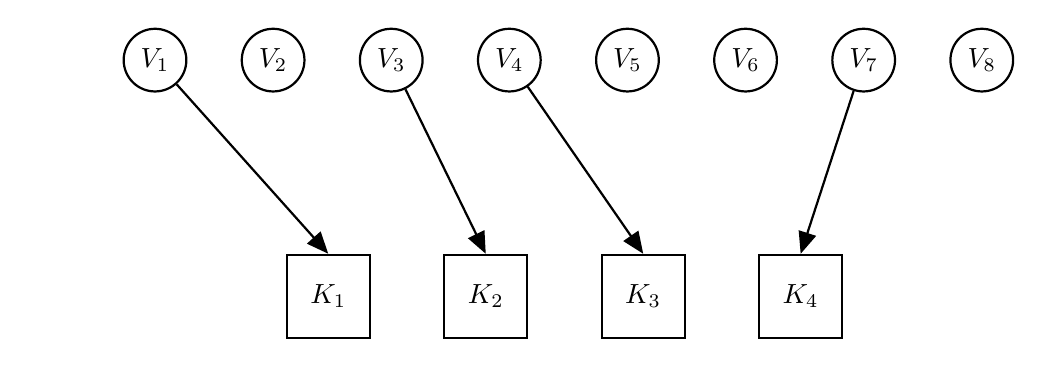
\begin{tikzpicture}[auto, thick, node distance=2cm, >=triangle 45]
        \draw
        node at(0,0)[name=start1]{}
        node [sum, name=VThread1, right of=start1]{$V_1$}
        node [sum, name=VThread2, right of=VThread1]{$V_2$}
        node [sum, name=VThread3, right of=VThread2]{$V_3$}
        node [sum, name=VThread4, right of=VThread3]{$V_4$}
        node [sum, name=VThread5, right of=VThread4]{$V_5$}
        node [sum, name=VThread6, right of=VThread5]{$V_6$}
        node [sum, name=VThread7, right of=VThread6]{$V_7$}
        node [sum, name=VThread8, right of=VThread7]{$V_8$};
        \draw
        node at(1.7,-3)[name=start2]{}
        node [block, name=Kern1, right of=start2]{$K_1$}
        node [block, name=Kern2, right of=Kern1]{$K_2$}
        node [block, name=Kern3, right of=Kern2]{$K_3$}
        node [block, name=Kern4, right of=Kern3]{$K_4$};
        \draw[->](VThread1) -- node{} (Kern1.north);
        \draw[->](VThread3) -- node{} (Kern2.north);
        \draw[->](VThread4) -- node{} (Kern3.north);
        \draw[->](VThread7) -- node{} (Kern4.north);
    \end{tikzpicture}
    \caption{Aufteilung von Virtuellen Threads auf Kernel}
\end{figure}

\subsection{Aufbau von Prozessen}

Prozesse müssen noch ein wenig mehr als nur ein Stück Quelltext besitzen, um aktiv zu werden. Generell kann man sagen, dass Prozesse aus 7 Elementen bestehen.
Diese nennt man Prozesskontext. Innerhalb des Prozesskontextes gibt es noch den Hardwarekontext. Er besteht aus folgendem:
\begin{itemize}
    \setlength\itemsep{0pt}
    \item Das auszuführende Programm
    \item Die Daten des Programms: umfasst unter anderen die globalen Variablen
    \item Einem Stack: ein Stack funktioniert nach dem push und pop Verfahren und speichert die lokalen Variablen für einen schnelleren Zugriff
    \item Kernelstack: umfasst die Systemaufrufe des Prozesses
          \begin{itemize}
              \item CPU Register: kann in den meisten Fällen nur ein Befehl speichern (64bit Prozessor = 64bits im Register)
              \item MMU Register: verwaltet den Zugriff auf den Arbeitsspeicher
          \end{itemize}
\end{itemize}

Da ein Prozess viele Kontextwechsel durchleben wird, muss das Betriebssystem bestimmte Register speichern. Dazu gehört aus dem Hardwarekontext:

\begin{itemize}
    \setlength\itemsep{0pt}
    \item Instruction Pointer - die Speicheradresse des nächsten Befehls
    \item Instruction Register - der aktuelle Befehl
    \item Stackpointer - speichert das Ende des Stacks
    \item Basepointer - Speicheradresse des aktuellen Elements im Stack
    \item Akkumulator - speichert Ergebnisse der ALU
\end{itemize}

Dies sind die wichtigsten Informationen, um die Rechenoperationen weiterführen zu können. Das Betriebssystem braucht noch weitere Informationen über einen Prozess. Sie werden auch Systemkontext genannt. Die wichtigsten davon sind:

\begin{itemize}
    \setlength\itemsep{0pt}
    \item Ort in der Prozesstabelle
    \item PID - Prozessnummer
    \item Prozesszustand
    \item Priorität
    \item Eltern- oder Kindprozesse
    \item Zugriffsrechte - Linux: -20 bis 19
    \item Erlaubte Ressourcenmengen - bsp. Maximaler RAM Verbrauch
    \item Verwendete Dateien - um zu verhindern, dass mehre Prozesse an einer Datei arbeiten
    \item Zugeordnete Geräte - Maus, Tastatur, ...
\end{itemize}

Mithilfe der Prozesstabelle kann das Betriebssystem die einzelnen Prozesse speichern. In dieser werden Prozesskontrollblöcke gespeichert, welche den Hardwarekontext und Systemkontext beinhalten. Bei einem Kontextwechsel wird der Prozesskontext aus der Prozesstabelle wieder hergestellt.

\newpage

\subsection{Verwalten der Prozesse}

Jedes Betriebssystem muss einen Weg haben, um effektiv die Kontextwechsel der Prozesse durchführen zu können. Dazu wird in den meisten Fällen ein Warteschlangen System, siehe Abbildung \ref{Warteschlange Prozesse}, verwendet. Auch hat ein Prozess deutlich mehr Zustände in einem modernen Betriebssystem als nur \textit{untätig} und \textit{rechnend}. Dazu wird heutzutage meistens das Prozessmodell wie in Abbildung \ref{Prozessmodell} oder eine modifizierte Variante verwendet. Linux als Beispiel verwendet ein \textit{8-Zustands Prozessmodell}, welches das Modell mit einem \textit{kernel rechnend} Zustand erweitert.

\begin{figure}[h]
    \centering
    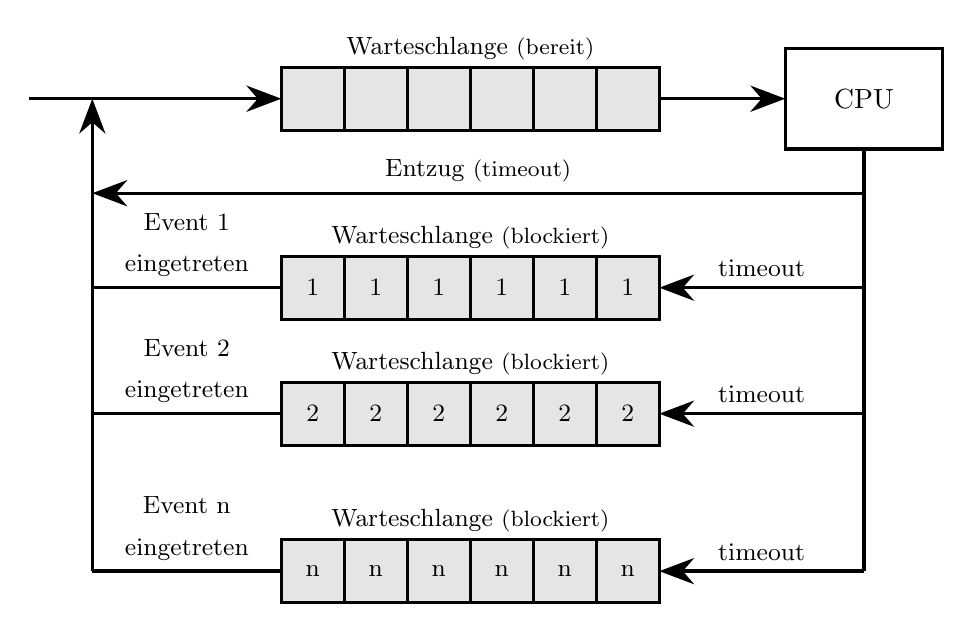
\begin{tikzpicture}[y=-1cm, scale=0.8]
    \pgfmathsetmacro\start{2}
    \pgfmathsetmacro\endValue{5}
    \draw[very thick, -{Stealth[scale=1.5]}](-2,1.5) -- (\start,1.5);

    %Warteschlange
    \foreach \x in {0,...,\endValue}{
        \filldraw[very thick, draw = black, fill = black!10](\start+\x, 1) rectangle (\start+\x+1, 2);
    }

    \pgfmathsetmacro\middleLine{\start+((\endValue+1)/2)}
    \node[align=center] at (\middleLine, 0.7){\small Warteschlange \footnotesize(bereit)};

    \draw[very thick, -{Stealth[scale=1.5]}](\start+\endValue+1,1.5) -- (\start+\endValue+3,1.5);

    \draw[very thick, draw = black](\start+\endValue+3, 0.7) rectangle (\start+\endValue+3+2.5, 2.3) node[pos=.5] {CPU};

    %Linien
    \pgfmathsetmacro\middleCPU{\start+\endValue+3+1.25}
    \pgfmathsetmacro\endLine{\start+\endValue+1}

    \draw[very thick](\middleCPU, 2.3) -- (\middleCPU, 9);
    \draw[very thick, -{Stealth[scale=1.5]}](-1, 9) -- (-1, 1.5);

    %Entzug der CPU
    \draw[very thick, -{Stealth[scale=1.5]}](\middleCPU, 3) -- (-1, 3) node [midway, above] {\small Entzug \footnotesize (timeout)};

    %Event 1
    \draw[very thick, -{Stealth[scale=1.5]}](\middleCPU, 4.5) -- (\endLine, 4.5) node [midway, above] {\small timeout};
    \foreach \x in {0,...,\endValue}{
        \filldraw[very thick, draw = black, fill = black!10](\start+\x, 4) rectangle (\start+\x+1, 5) node[pos=.5] {\small 1};
    }
    \node[align=center] at (\middleLine, 3.7){\small Warteschlange \footnotesize(blockiert)};
    \draw[very thick](\start, 4.5) -- (-1, 4.5) node [midway, above, align=center] {\small Event 1\\\small eingetreten};

    %Event 2
    \draw[very thick, -{Stealth[scale=1.5]}](\middleCPU, 6.5) -- (\endLine, 6.5) node [midway, above] {\small timeout};
    \foreach \x in {0,...,\endValue}{
        \filldraw[very thick, draw = black, fill = black!10](\start+\x, 6) rectangle (\start+\x+1, 7) node[pos=.5] {\small 2};
    }
    \node[align=center] at (\middleLine, 5.7){\small Warteschlange \footnotesize(blockiert)};
    \draw[very thick](\start, 6.5) -- (-1, 6.5) node [midway, above, align=center] {\small Event 2\\\small eingetreten};

    %Event n
    \draw[very thick, -{Stealth[scale=1.5]}](\middleCPU, 9) -- (\endLine, 9) node [midway, above] {\small timeout};
    \foreach \x in {0,...,\endValue}{
        \filldraw[very thick, draw = black, fill = black!10](\start+\x, 8.5) rectangle (\start+\x+1, 9.5) node[pos=.5] {\small n};
    }
    \node[align=center] at (\middleLine, 8.2){\small Warteschlange \footnotesize(blockiert)};
    \draw[very thick](\start, 9) -- (-1, 9) node [midway, above, align=center] {\small Event n\\\small eingetreten};
\end{tikzpicture}
    \caption{Warteschlangensystem\protect\footnotemark}
    \label{Warteschlange Prozesse}
\end{figure}
\footnotetext{Grafik in Anlehnung an \cite[Seite 154]{BetriebssystemeKompakt}}
\begin{figure}[h]
    \centering
    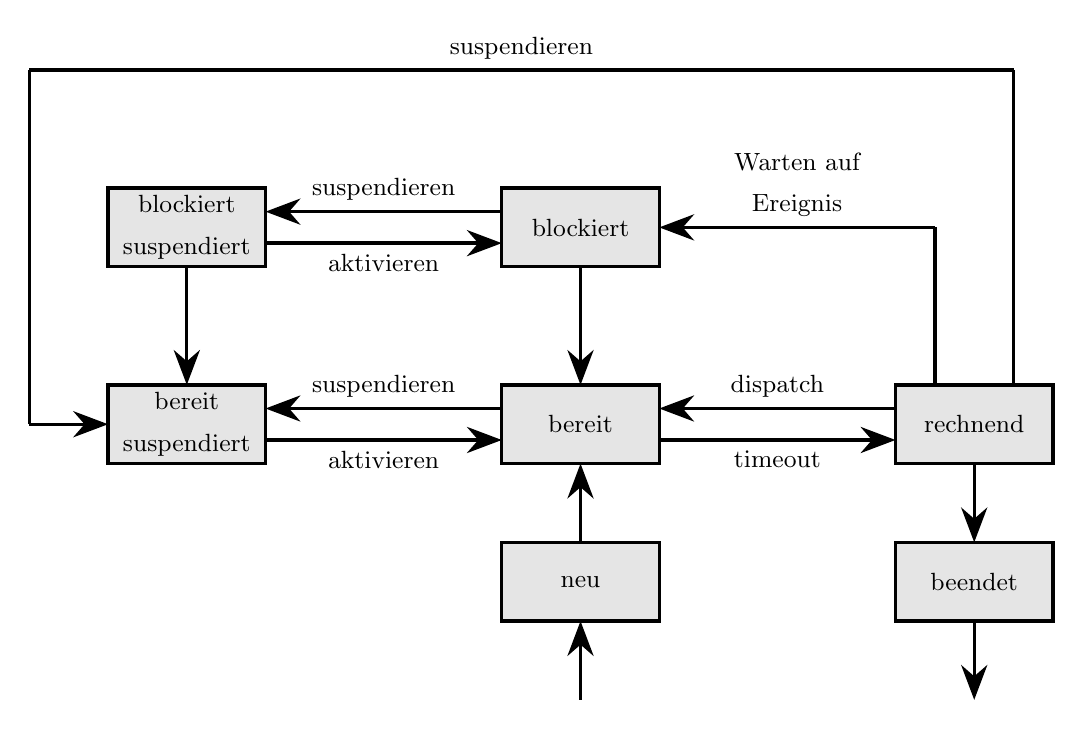
\begin{tikzpicture}
    %neu
    \draw[very thick, -{Stealth[scale=1.5]}](7, 1) -- (7, 2);
    \filldraw[very thick, draw = black, fill = black!10](6, 3) rectangle (8, 2) node[pos=.5] {\small neu};

    %bereit
    \draw[very thick, -{Stealth[scale=1.5]}](7, 3) -- (7, 4);
    \filldraw[very thick, draw = black, fill = black!10](6, 5) rectangle (8, 4) node[pos=.5] {\small bereit};
    \draw[very thick, -{Stealth[scale=1.5]}](8, 4.3) -- (11, 4.3) node [midway, below] {\small timeout};
    \draw[very thick, -{Stealth[scale=1.5]}](6, 4.7) -- (3, 4.7) node [midway, above] {\small suspendieren};

    %blockiert
    \draw[very thick, -{Stealth[scale=1.5]}](7, 6.5) -- (7, 5);
    \filldraw[very thick, draw = black, fill = black!10](6, 7.5) rectangle (8, 6.5) node[pos=.5] {\small blockiert};
    \draw[very thick, -{Stealth[scale=1.5]}](6, 7.2) -- (3, 7.2) node [midway, above] {\small suspendieren};
    
    %beendet
    \filldraw[very thick, draw = black, fill = black!10](11, 3) rectangle (13, 2) node[pos=.5] {\small beendet};
    \draw[very thick, -{Stealth[scale=1.5]}](12, 2) -- (12, 1);

    %rechnend
    \draw[very thick, -{Stealth[scale=1.5]}](12, 4) -- (12, 3);
    \filldraw[very thick, draw = black, fill = black!10](11, 5) rectangle (13, 4) node[pos=.5] {\small rechnend};
    \draw[very thick, -{Stealth[scale=1.5]}](11, 4.7) -- (8, 4.7) node [midway, above] {\small dispatch};
    \draw[very thick](11.5, 5) -- (11.5, 7);
    \draw[very thick, -{Stealth[scale=1.5]}](11.5, 7) -- (8, 7) node [midway, above, align=center] {\small Warten auf \\\small Ereignis};
    \draw[very thick](12.5, 5) -- (12.5, 9);
    \draw[very thick](12.5, 9) -- (0, 9) node [midway, above] {\small suspendieren};
    \draw[very thick](0, 9) -- (0, 4.5);
    \draw[very thick, -{Stealth[scale=1.5]}](0, 4.5) -- (1, 4.5);

    %bereit suspendiert
    \filldraw[very thick, draw = black, fill = black!10](1, 5) rectangle (3, 4) node[pos=.5, align=center] {\small bereit\\\small suspendiert};
    \draw[very thick, -{Stealth[scale=1.5]}](3, 4.3) -- (6, 4.3) node [midway, below] {\small aktivieren};

    %blockiert suspendiert
    \filldraw[very thick, draw = black, fill = black!10](1, 7.5) rectangle (3, 6.5) node[pos=.5, align=center] {\small blockiert\\\small suspendiert};
    \draw[very thick, -{Stealth[scale=1.5]}](2, 6.5) -- (2, 5);
    \draw[very thick, -{Stealth[scale=1.5]}](3, 6.8) -- (6, 6.8) node [midway, below] {\small aktivieren};
\end{tikzpicture}
    \caption{7-Zustands Prozessmodell\protect\footnote{eine fußnote}}
    \label{Prozessmodell}
\end{figure}

\newpage
\footnotetext{Grafik in Anlehnung an \cite[Seite 156]{BetriebssystemeKompakt}}

Wie in der Einleitung schon angesprochen sind die Zustände \textit{bereit} und \textit{rechnend} die wichtigsten Zustände. Mit diesen alleine könnte ein Betriebssystem funktionieren. In diesem System gibt es nur eine Warteschlange, in der sich alle Prozesse des Zustandes \textit{bereit} befinden. Idealer Weise implementiert der \textit{Scheduler}\footnote{Programm zum Managen der Warteschlangen.} einen Algorithmus, welcher die Priorität der Prozesse berücksichtigt. Wie schon erwähnt muss sich der \textit{Dispatcher}\footnote{Programm zum Ausführen der Prozesswechsel.} um noch weitere Zustände kümmern. Diese und ihre Beziehungen sind in Grafik \ref{Prozessmodell} zu finden. Zwei davon wären \textit{neu} und \textit{beendet}. Diese sind für eine größere Flexibilität nützlich. Mit dem \textit{beendet}-Zustand, können Informationen nachträglich von einem fertigen Prozess aufgerufen werden. Der Zustand \textit{neu} hat die gemeinsame Funktion mit dem \textit{beendet}-Zustand Ressourcen zu sparen.\newline
Ein entscheidender Fehler ist es anzunehmen, dass alle Prozesse jederzeit arbeiten wollen. So könnte ein Programm auf eine Tastatur Eingabe oder andere Ereignisse warten. Um diese Funktionalität bereitzustellen, gibt es den Zustand \textit{blockiert}. In diesen wechselt ein Prozess nach dem berechnen und kann aus diesen sich wieder in die Warteschlange der \textit{bereiten}-Prozesse einordnen. In Grafik \ref{Warteschlange Prozesse} werden unterschiedliche Warteschlangen für unterschiedliche Ereignisse erzeugt. Dieses Vorgehen hat den Vorteil gegenüber einer einzelnen ``blockiert-Warteschlange'', dass häufig genutzte Events wie Tastenanschläge nicht von seltenen Events beeinträchtigt werden.\newline
Da es sehr schnell zu vielen Prozessen kommen kann, wird mit den Zuständen \textit{blockiert suspendiert} und \textit{bereit suspendiert} eine Möglichkeit geschaffen, selten genutzte Prozesse aus dem Arbeitsspeicher in den Massenspeicher\footnote{Spezielle Partitionen auf einer Festplatte. Auch \textit{swap} genannt.} zu verschieben. Wie die Namen schon implizieren werden Prozesse in den Zuständen \textit{blockiert} und \textit{bereit} jeweils suspendiert und aktiviert. Für zusätzliche Geschwindigkeit können Prozesse selbst im suspendierten Zustand auf Ereignisse reagieren und von \textit{blockiert suspendiert} in \textit{bereit suspendiert} wechseln. Es gibt demnach ein zweites \captionref{Warteschlange Prozesse} für die suspendierten Prozesse. Dieses beinhaltet keinen ?Zugriff auf die CPU, sondern kann die Prozesse maximal aktivieren und in den Arbeitsspeicher verschieben. \cite{BetriebssystemeKompakt}

\newpage

\subsection{Funktionsweise des Schedulers}
Der \textit{Scheduler} ist ein sehr wichtiges und mächtiges Stück Quelltext. Es regelt alle anderen Prozesse eines Betriebssystems. Es kann sich die Frage gestellt werden, wie der \textit{Scheduler} ausgeführt wird. Ist er nur ein weiterer Prozess? Dies würde aber implizieren, dass er sich selber managen würde. Oder wird er auf einem eigenen CPU Kern ausgeführt? Aber Linux läuft doch auch auf einem einzelnem Kern. Die Antwort liegt in der Natur des Kernels.
\medskip
\newline
Der Kernel ist die niedrigste Instanz mit der höchsten Berechtigung in einem System. Nichts steht zwischen ihm und der CPU. Jedes Programm muss über den Kernel um arbeiten zu können. Der \textit{Scheduler} ist ein Teil des Kernels. Der Kernel ist jedoch kein einzelner Prozess, welcher immer läuft, sondern eine Art Bibliothek. Ein Programm wendet sich an den Kernel und nicht der Kernel an das Programm. Dementsprechend läuft der \textit{Scheduler} nicht dauerhaft, sondern wird extern getriggert. Der \textit{Scheduler} wird entweder von einem beendeten Prozess oder nach einer Zeitunterbrechung getriggert. Die Zeitunterbrechung wird dabei von der CPU durch den \textit{programmable interrupt timer (PIT)} erzeugt und im Kernel durch den \textit{timer interrupt handler} aufgefangen, welcher auch den \textit{Scheduler} startet. Es wird dabei zwischen einem \textit{ticked kernel} und \textit{tickless kernel} unterschieden. Bei dem \textit{ticked kernel} ist der Zeitintervall immer gleich, wogegen der des \textit{tickless kernels} dynamisch verändert werden kann.\cite{tickles:Love}
\bigskip
\newline
Der \textit{Scheduler} verwaltet die einzelnen Warteschlangen und entscheidet, wann ein Prozess auf die CPU zugreifen darf. Dabei ist es wichtig die beste Effizienz beizubehalten und trotzdem eine gute Verteilung der Prozesszeit zu ermöglichen. Denn Kontextwechsel sind aufwändig. Bei vielen kleinen Prozessen wird viel Zeit für das Speichern der Register und das Wiederherstellen eines Prozesses aus der \textit{Prozesstabelle} verwendet. Je länger ein Prozess arbeiten kann, desto effizienter wird die Zeit genutzt. Daher haben sich zwei grundlegende Konzepte des \textit{schedulings} gebildet. Diese Schedulingverfahren sind:
\begin{itemize}
    \item \textit{Nicht-präemptives Scheduling}. Bei diesem hat ein Prozess, bis zu seiner Fertigstellung, volle Kontrolle über die CPU. Der \textit{Scheduler} führt erst den Kontextwechsel nach dessen Vollendung aus. Es kann Situationen geben, bei denen ein Prozess sich nicht selber beendet. Beispielsweise durch eine Endlosschleife in der Programmierung oder der Entwickler setzt bei der Programmierung das \textit{Präemtive Scheduling} voraus.
    \item \textit{Präemtives Scheduling}. Dieses wird seit Windows 3.x und Mac OS8/9 verwendet. Dabei wird nicht auf die Vollendung eines Prozesses gewartet, sondern kann und wird in den meisten Fällen, der Prozess der CPU vor Beendung entzogen. Der Vorteil ist, dass viele weitere Prozesse ``gleichzeitig'' arbeiten können, ohne dass der Nutzer das ``Einfrieren'' anderer Prozesse erfährt. Der Nachteil dabei ist, dass die Kontextwechsel viel Zeit in Anspruch nehmen. Somit haben die Prozesse weniger Arbeitszeit und die gesamte Leistung der CPU sinkt etwas. Da die Vorteile der größeren Freiheit der leicht verringerten Leistung überwiegen, wird dieses Verfahren in den meisten modernen Betriebssystemen verwendet. \cite{BetriebssystemeKompakt}
\end{itemize}

Auf diesen zwei grundlegenden Systemen haben sich weitere \textit{Scheduling} Verfahren entwickelt, welche das Verwalten der Warteschlange implementieren. Um ein ideales System zu erschaffen, müssen bestimmte Punkte berücksichtigt werden. Es lassen sich nicht immer alle Kriterien miteinander vereinbaren und es ist dem Entwickler überlassen, welche er bevorzugt. Die Kriterien wären wie folgt: \cite{Scheduling:Williams}
\begin{itemize}
    \item Prozessor-Auslastung - die Prozessor-Auslastung sollte im Idealfall so hoch wie möglich sein, damit kein Befehlszyklus\footnote{Ein Befehlszyklus ist der kleinste Zeitintervall einer CPU. Befehle können unterschiedlich viele Befehlszyklen brauchen. Je kleiner der Befehlszyklus ist, desto höher ist die Hertz Anzahl einer CPU} verschwendet wird
    \item Antwortzeit - die Zeit, die vergeht, bis die erste Antwort eines Prozesses nach Anfrage ankommt
    \item Durchlaufzeit - die Zeit, die vergeht, bis ein Prozess nach Einreichung beendet ist
    \item Durchsatz - wie viele Prozesse in einem vorgegebenen Intervall beendet werden. Der Intervall kann je nach Anwendungsfall variieren
    \item Wartezeit - die Zeit, die ein Prozess in der bereit-Warteschlange verbringt, bis er zugriff auf die CPU bekommt
    \item Fairness - die Fairness eines Verfahren bestimmt, wie gut kleine und weniger priorisierte Prozesse eine Chance haben Prozesszeit zu erhalten
\end{itemize}

Im Folgenden werde ich zwei \textit{Scheduling} Verfahren vorstellen.
\newpage
\subsubsection{Completetely Fair Scheduling}
\textit{Completetely Fair Scheduling}\footnote{\textit{Completetely Fair Scheduling (CFS)} wurde 2007 das erste Mal von Ingo Molnar im Linux Kernel eingearbeitet.} ist, wie der Name schon impliziert, eine Form des \textit{Ideal Fair Scheduling}. Es besagt, dass versucht wird die Prozesse gleich lange Arbeiten zu lassen. In den Tabellen \ref{Fair Scheduling} sind vier Prozesse dargestellt. Alle haben die selbe Priorität. In dem Szenario hat jeder Zeit-Quant($Q_1$, $Q_2$, \dots) eine Zeitspanne von 4ms. In den ersten vier Quanten bekommt jeder Prozess 1ms. Ab $Q_4$ sind Prozess B und D abgeschlossen und A und C erhalten somit in $Q_5$ jeweils 2ms. Durch das Prinzip werden alle Prozesse gleich behandelt. \cite[Ab 1:35]{CFS:Rebeiro}
\begin{figure}[h]
    \centering
    \begin{tabular}{| l | l |}
        \hline
        Prozess & Ausführungszeit\\
        \hline
        A & 8ms\\
        \hline
        B & 4ms\\
        \hline
        C & 16ms\\
        \hline
        D & 4ms\\
        \hline
    \end{tabular}
    \begin{tabular}{| x{1em} | x{1em} | x{1em} | x{1em} | x{1em} | x{1em} | x{1em} | x{1em} | x{1em} |}
        \hline
        \rowcolor{black!10}
        & $Q_1$ & $Q_2$ & $Q_3$ & $Q_4$ & $Q_5$ & $Q_6$ & $Q_7$ & $Q_8$\\
        \hline
        \rowcolor{black!20}
        A & 1 & 2 & 3 & 4 & 6 & 8 & &\\
        \hline
        \rowcolor{black!10}
        B & 1 & 2 & 3 & 4 & & & &\\
        \hline
        \rowcolor{black!20}
        C & 1 & 2 & 3 & 4 & 6 & 8 & 12 & 16\\
        \hline
        \rowcolor{black!10}
        D & 1 & 2 & 3 & 4 & & & &\\
        \hline
    \end{tabular}
    \captionof{table}{\textit{Fair Scheduling (FS)}\protect\footnote{eine fußnote}}
    \label{Fair Scheduling}
\end{figure}
\footnotetext{Grafik in Anlehnung an \cite[Minute 1:35]{CFS:Rebeiro}}

Im CFS wird das Prinzip des FS nicht hauptsächlich mit Zeitscheiben gelöst. Es wird das Konzept der \textit{vruntime} eingebracht. \textit{Vruntime} bedeutet dabei, wie lange ein Prozessor bereits ausgeführt wurde. CFS berechnet weiterhin unterschiedliche Zeitscheiben für die PIT, jedoch werden diese zur Maximierung der Effizienz genutzt. Prozesse mit komplexen Rechnungen sind effizienter, wenn sie mehr Zeit ohne Kontextwechsel haben. Prozesse wie Tracker\footnote{Programm um etwas aufzuzeichnen (Bspw. Anzahl der Tastenanschläge)} schadet der Kontextwechsel nicht allzu sehr. Der \textit{Scheduler} addiert auf die alte \textit{vruntime} die Zeit $\Delta t$, die der Prozessor lief. Sollte der Prozess noch nicht abgeschlossen sein, wird die neue \textit{vruntime} in einen Rot-Schwarz Baum eingefügt. Ein Rot-Schwarz Baum ist ein Binärbaum, welcher eine selbst ausgleichende Natur besitzt. Somit beträgt die einfüge Laufzeit $\mathcal{O}(\log n)$. CFS wählt als nächsten Prozess, den mit der geringsten \textit{vruntime} aus. Dabei wird immer ein Pointer auf das kleinste Blatt gehalten, um mit einer Laufzeit von $\mathcal{O}(1)$ den Prozess mit der kleinsten \textit{vruntime} zu finden. Durch das Wählen der kleinsten \textit{vruntime} wird das Prinzip des \textit{Fair Schedulings} eingehalten. \cite[Ab 5:22]{CFS:Rebeiro}
\medskip
\newpage
Das Nutzen der \textit{vruntime} als zentralen Wert hat weitere Vorteile. So können die Prioritäten ohne Umwege eingearbeitet werden. Der CFS verwaltet in der \textit{vruntime} drei unterschiedliche \textit{Scheduling Policies}. \cite{LinuxDoc:Torvalds}
\begin{itemize}
    \item \textbf{SCHED\_NORMAL/SCHED\_OTHER} - die normale Regel für Prozesse
    \item \textbf{SCHED\_BATCH} - für Prozesse, die nicht interaktiv sind und den Arbeitsbereich des Nutzers nicht stören wollen
    \item \textbf{SCHED\_IDLE} - die niedrigste Regel für Prozesse und sie werden an wenigsten bevorzugt
\end{itemize}
SCHED\_NORMAL und SCHED\_BATCH sind zusätzlich von den \textit{nice} Werten abhängig. Die \textit{nice} Werte reichen von -20 bis 19 und repräsentieren die Priorität eines Prozesses. Je kleiner der \textit{nice} Wert, desto höher ist die Priorität\cite{Scheduler:Kerrisk}. Dabei ist der Unterschied linear. Die Verteilung des Prozessors auf zwei Prozesse mit \textit{nice} Werten von 11 und 12, wäre 55\% und 45\%. Bei Prozessen mit -4 und -5 bleibt die Verteilung gleich. Die neue \textit{vruntime} wird mit Formel \ref{calc_vruntime}\cite{LinuxKernel:Torvalds} berechnet.
\begin{align}
    \text{vruntime} \mathrel{+}= \text{delta\_exec} \cdot \frac{\text{weigth}}{\text{lw.weight}}
    \label{calc_vruntime}
\end{align}
Dabei ist \textit{weigth} mit 1024 oder \textit{nice\_0} definiert. \textit{lw.weigth} ist die Priorität als \textit{weigth}. Das kann aus dem Array in dem Listing \ref{core.c}\cite{LinuxKernel:Torvalds} entnommen werden.
\begin{figure}[h]
    \centering      
    \lstset{
    language=C,
    keywordstyle=\color{blue},
    commentstyle=\color{green},
    }
    \begin{tabular}{c}
        \begin{lstlisting}{Latexkernel core.c}
10886 const int sched_prio_to_weight[40] = {
10887 /* -20 */ 88761, 71755, 56483, 46273, 36291,
10888 /* -15 */ 29154, 23254, 18705, 14949, 11916,
10889 /* -10 */ 9548,  7620,  6100,  4904,  3906,
10890 /*  -5 */ 3121,  2501,  1991,  1586,  1277,
10891 /*   0 */ 1024,  820,   655,   526,   423,
10892 /*   5 */ 335,   272,   215,   172,   137,
10893 /*  10 */ 110,   87,    70,    56,    45,
10894 /*  15 */ 36,    29,    23,    18,    15,
10895 };
        \end{lstlisting}
    \end{tabular}
    \captionof{lstlisting}{Linuxkernel core.c{\footnotesize (v5.17-rc3)} \textit{nice} Werte als \textit{weigth}}
    \label{core.c}
\end{figure}
\newpage

\subsubsection{Round Robin}
Das Round Robin(RR) Verfahren ist weitverbreitet. Es wird in abgewandelter Form auch heutzutage in Windows verwendet.\cite{Windows:Lohmann} Das RR \textit{Scheduling} nutzt Zeitquanten. Diese Befinden sich meistens im ein- oder zweistelligen Millisekundenbereich. Jeder Prozess wird nacheinander für die Länge des Zeitquanten ausgeführt und danach dem Prozessor entzogen. Ist der Prozess früher beendet, wird ein neuer Zeitquant eingeleitet. Ist der Prozess nicht beendet, wird er wieder in die Warteschlange am Ende angehängt.\cite[Seite 176f.]{BetriebssystemeKompakt}\\
\begin{figure}[h]
    \centering
    \begin{tabular}{| l | l |}
        \hline
        Prozess & Ausführungszeit\\
        \hline
        \cellcolor{red!20}A & 30ms\\
        \hline
        \cellcolor{blue!20}B & 50ms\\
        \hline
        \cellcolor{green!20}C & 20ms\\
        \hline
        \cellcolor{black!20}D & 30ms\\
        \hline
    \end{tabular}
    \begin{tabular}{|c|c|c|c|c|c|c|c|c|c|c|c|c|c|c|c|c|c|c|c|c|}
        \hline
        \cellcolor{red!20} & \cellcolor{red!20} & \cellcolor{blue!20} & \cellcolor{blue!20} & \cellcolor{green!20} & \cellcolor{green!20} & \cellcolor{black!20} & \cellcolor{black!20} & \cellcolor{red!20} & \cellcolor{blue!20} & \cellcolor{blue!20} & \cellcolor{black!20} & \cellcolor{blue!20}\\
        \hline
        \multicolumn{1}{l}{} & \multicolumn{2}{c}{\tiny 20} & \multicolumn{2}{c}{\tiny 40} & \multicolumn{2}{c}{\tiny 60} & \multicolumn{2}{c}{\tiny 80} & \multicolumn{2}{c}{\tiny 100} & \multicolumn{2}{c}{\tiny 120}\\
    \end{tabular}
    \caption{Round Robin Beispiel}
    \label{RoundRobin}
\end{figure}

In \ref{RoundRobin} werden vier Prozesse in der vorgegebenen Reihenfolge abgearbeitet. Die Zeitquanten in dem Beispiel sind 20ms lang. Prozess C benötigt nur ein Zeitquanten und wird beendet. Prozesse A und D benötigen 1.5 Zeitquanten. Sie arbeiten beim zweiten Mal nur 10ms und der nächste Prozess kann nachrücken. Prozess B benötigt am meisten Zeit und wird dreimal ausgeführt. Erst beim dritten Mal kann er beendet werden.
\medskip
\newline
Das Round Robin Verfahren kann noch mit Prioritäten erweitert werden. Dieses werde ich am Beispiel des \textit{Schedulers} von Windows erklären. Windows verwendet ein prioritätengesteuertes \textit{Scheduling}\footnote{Die Prioritäten von Windows reichen dabei von 0 bis 31}. Das RR Verfahren wird dabei immer auf die selbe Priorität angewendet. Die höhere Priorität wird immer bevorzugt. Dazu wird für jede Priorität eine eigene Warteschlange angelegt. Um das Verhungern eines Prozesses zu verhindern, nutzt Windows noch variable Prioritäten. Bei den variablen Prioritäten hat Windows noch die Möglichkeit selber zu ermitteln welche Prozesse wichtiger sind.\cite[Folie 9-12]{Windows:Lohmann}
\medskip
\newline
Mit dem Round Robin Verfahren kann grundsätzlich eine faire Umgebung geschaffen werden. Werden jedoch Prioritäten ohne Variation bevorzugt, kann es zu einem unfairen System werden. Auch sind I\/O-lastige\footnote{I\/O = Input\/Output. Ein Prozess wartet z.B. auf eine Eingabe des Benutzers.} Prozesse benachteiligt. Sie benötigen selber nur wenig Ausführungszeit, müssten aber für das reibungslose Funktionieren häufiger Zugriff auf den Prozessor erhalten. Im Round Robin \textit{Scheduling} müssen sie warten, bis rechenintensive Prozesse den Zeitquanten vollständig verbrauchen, bevor sie wieder an der Reihe sind.

\subsection{Threads}\label{Threads}
In modernen Computer Systemen gibt es noch Threads neben Prozessen. Threads sind dabei deutlich häufiger vertreten als Prozesse. Auf meinem Computer laufen durchschnittlich 20x mehr Threads als Prozesse. Dies liegt daran, dass Threads als Prozess eines Prozesses gesehen werden. Ein Programm ist nur ein Prozess, kann aber viele eigene Threads besitzen. Die Funktionalität von Threads unterscheidet sich nicht viel von Prozessen. Sie werden im \textit{Scheduler} gleich behandelt und es gibt nur geringe Unterschiede bei dem Kontextwechsel.
\medskip
\newline
Threads haben jedoch ein paar Besonderheiten gegenüber Prozessen. Denn im Gegensatz zu Prozessen, welche unabhängig voneinander laufen, haben Threads diese Beschränkung nicht. Es liegt daran, dass Threads auf den Stack des Prozesses zugreifen können. Threads teilen sich somit die globalen Variablen des Prozesses, speichern aber eigene lokale Variablen im eigenen Stack. Aufgrund diesem Prinzip können mehrere Threads mit dem selben Quelltext arbeiten, ohne sich gegenseitig zu behindern.\cite{Threads:Williams}
\begin{figure}[h]
    \centering
    \input{images/Threads/ThreadinProzess.tex}
    \caption{Threads}
\end{figure}
\\Threads werden als Teil eines Prozesses betrachtet. Deswegen sind sie viel leichtgewichtiger und können schneller erstellt und beendet werden. Zusätzlich werden Threads in zwei Kategorien unterteilt.
\begin{itemize}
    \item \textbf{Nutzer Level Threads} werden mithilfe einer Thread-library implementiert und sind unabhängig von dem Betriebssystem. Infolge können Nutzer Level Threads auch auf einem System ohne unterstütztem Multiprozessing in Betrieb genommen werden. Außerdem ist das Management von vielen Threads schneller, da keine Systemaufrufe getätigt werden müssen.
    \item \textbf{Kernel Level Threads} werden vom Betriebssystem implementiert und auch von diesem verwaltet. Dadurch ergeben sich Vorteile, wie auch Nachteile. Ein Vorteil wäre, dass Prozesse mit einer hohen Thread Anzahl bevorzugt werden könnten. Der Nachteil ist, dass die Verwaltung auf Kernel Ebene deutlich intensiver ist. Auch muss für jeden Thread ein einzelner Kontrollblock erstellt werden. \cite{Threads:Dusey}
\end{itemize}
\subsection{Threads in Java}
In Java sind Threads auf dem Kernel Level implementiert. In Versionen vor 1.2(1998) gab es die so genannten grünen Threads. Diese waren Nutzer Level Threads und in der Java VM implementiert. Heutzutage nutzt Java Kernel Level Threads, welche den Vorteil haben die gesamte CPU zu nutzen. Ein Prozess mit mehreren Threads kann somit alle vorhandenen CPU Kerne benutzen. Im Modell der grünen Threads wurde dies über Umwege gelöst. So wurden die grünen Threads abwechselnd auf ein paar Kernel Level Threads verteilt, um mehrere Kerne nutzten zu können.\cite{Threads:Cox}
\subsubsection{Implementation in Java}
Threads werden in Java mithilfe der \textit{java.lang.Thread} Klasse verwirklicht. Es wird dabei zwischen zwei unterschiedlichen Implementierungen unterschieden.
\smallskip
\newline
\textbf{extends Thread:} Bei dieser Methode wird eine Klasse erstellt, welche die Thread Klasse erweitert. Der Vorteil dieses Vorgehens ist, dass alle Einstellungen innerhalb der neuen Klasse getätigt werden können.\cite{Java:Thread}
\lstset{
language=Java,
keywordstyle=\color{blue},
commentstyle=\color{green},
basicstyle=\linespread{0.8}\small,
}
\begin{figure}[h]
\begin{lstlisting}{extends Thread}
public class SimpleThread extends Thread {

    public SimpleThread(){
        super();
        //settings
        setPriority(Thread.NORM_PRIORITY);
    }

    @Override
    public void run(){
        System.out.println("Im Running");
    }

    public static void main(String[] args){
        SimpleThread t = new SimpleThread();
        t.start();
    }
}
\end{lstlisting}
\captionof{lstlisting}{mit Thread erweitern}
\end{figure}
\\Das Vorgehen hat seine Probleme. Denn es wird nicht die \textit{run()} Methode von Thread überschrieben, sondern die von Runnable, welches von Thread implementiert wird. Wenn die Thread Klasse erweitert wird, kann man keine weiteren Klassen erweitern. Um ein solches Problem zu lösen, kann auf die zweite Möglichkeit zurückgegriffen werden.
\smallskip
\newline
\textbf{implements Runnable:} Bei dieser Methode wird nicht ein selbständiger Thread erschaffen. Das Interface Runnable hat nur eine Methode - die \textit{run()} Methode.\cite{Java:Runnable} Um einen Thread zu starten, muss ein Thread Object erschaffen werden, welche im Konstruktor ein Object des interfaces Runnable erwartet.
\begin{figure}[h]
\begin{lstlisting}
public class SimpleRunnable implements Runnable{
    public SimpleRunnable(){

    }

    @Override
    public void run(){
        System.out.println("Im Running");
    }

    public static void main(String[] args){
        SimpleRunnable r = new SimpleRunnable();
        Thread t = new Thread(r);
        t.start();
    }
}
\end{lstlisting}
\captionof{lstlisting}{Runnable implementieren}
\end{figure}
\\Der Vorteil dieses Vorgehen ist, dass Runnable leichtgewichtiger ist und erst bei Ausführung ein Thread Object erschaffen wird. Auch ist die Separierung zwischen ``Aufgabe'' und ``Bearbeiter'' sinnvoll. Man erhält eine große Flexibilität. Es können zusätzlich Einstellungen an dem erschaffenen Thread Object vorgenommen werden. Die Methoden wie \textit{setPriority()} sind public.\cite{Java:Thread} Ein weiterer wichtiger Punkt ist, dass Runnables in einem Thread-Pool verwendet werden können.

\subsubsection{Thread-Pool}
Ein Thread-Pool ist wie eine zweite CPU nur in Software. Es gibt eine Warteschlange und eine festgelegte Anzahl an arbeitenden Threads. Der Unterschied ist, dass die Warteschlange nicht aus Threads besteht, sondern aus \textit{Runnables}. Diese werden auch nur ein einziges Mal ausgeführt und dabei nicht unterbrochen. Auch wird die Warteschlange chronologisch abgearbeitet. Ein Thread-Pool hat somit ein \textit{nicht-präemtives Scheduling}, welches mit dem \textit{first in first out} Verfahren arbeitet.\newpage
\begin{figure}[h]
    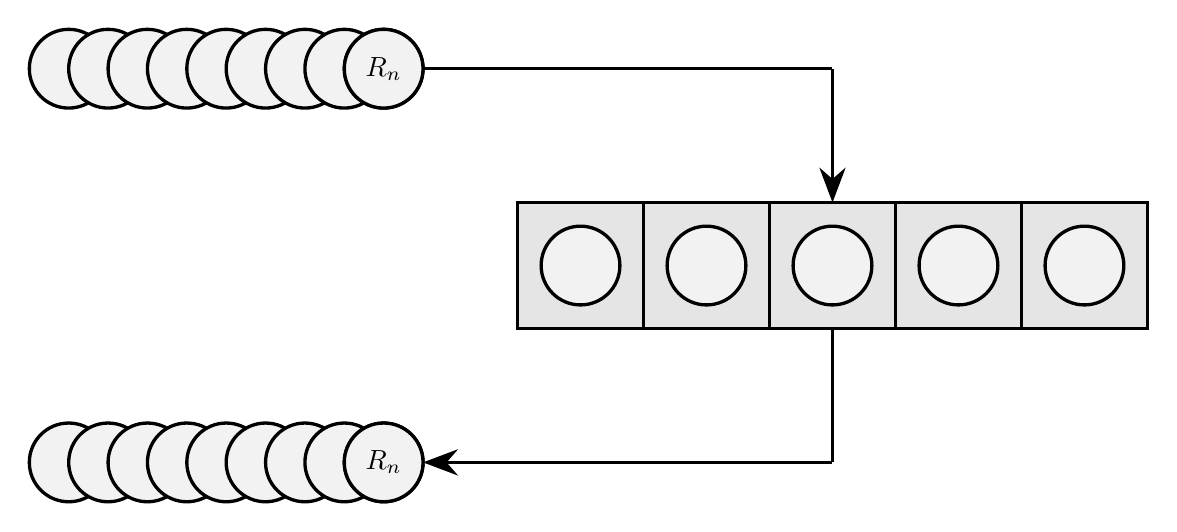
\begin{tikzpicture}
    \foreach \q in{0,0.5,...,4}{
        \filldraw[very thick, draw=black, fill=black!5](0+\q, 7) circle (0.5cm);
    }
    \draw[very thick](4, 7) -- (5.7+4, 7);
    \draw[very thick, -{Stealth[scale=1.5]}](5.7+4, 7) -- (5.7+4, 5.3);
    \filldraw[very thick, draw=black, fill=black!5](4, 7) circle (0.5cm) node[align=center] {$R_n$};

    \foreach \x in {0,1.6,...,8}{
        \filldraw[very thick, draw=black, fill=black!10](5.7+\x, 3.7) rectangle (7.3+\x, 5.3);
        \filldraw[very thick, draw=black, fill=black!5](6.5+\x, 4.5) circle (0.5cm);
    }

    \foreach \q in{0,0.5,...,4}{
        \filldraw[very thick, draw=black, fill=black!5](0+\q, 2) circle (0.5cm);
    }
    \draw[very thick](5.7+4, 3.7) -- (5.7+4, 2);
    \draw[very thick, -{Stealth[scale=1.5]}](5.7+4, 2) -- (4.5, 2);
    \filldraw[very thick, draw=black, fill=black!5](4, 2) circle (0.5cm) node[align=center] {$R_n$};
\end{tikzpicture}
    \caption{Thread-Pool\protect\footnotemark}
    \label{Thread-Pool}
\end{figure}
\footnotetext{Grafik in Anlehnung an \url{https://en.wikipedia.org/wiki/Thread_pool}}
In einem Thread-Pool werden die Aufgaben als \textit{Runnable} Object verwaltet. Eine bestimmte Anzahl an Threads arbeiten und erhalten immer neue \textit{Runnables}. Durch dieses Verfahren, muss nicht für jede Aufgabe ein neuer Thread erstellt werden. Auch ist ein Thread-Pool effizienter. Wenn viel berechnet werden muss, ist es besser weniger aktive Threads zu benutzten. Würden alle Aufgaben gleichzeitig gestartet werden, müsste der \textit{System Scheduler} die Threads verwalten. Es würden somit viel mehr Kontextwechsel stattfinden, bis alle Aufgaben abgearbeitet sind. Daher ist eine optimale Größe eines Thread-Pools in der Größenordnung der vorhandenen Kerne.\cite{ThreadPool:Java}

\subsubsection{Threadsicherheit}\label{Threadsicherheit}
\begin{center}
    \textit{
        [...]That the concept [of thread safety] itself is completely vague and essentially means nothing more than ``behaves correctly in some situations''[...]
    } - Eric Lippert \cite{Threads:Lippert}
\end{center}

Wie Herr Lippert in seinem Artikel bereits klarstellt, ist Threadsicherheit kein besonders kleines Thema. Auch ist Threadsicherheit immer im Auge des Betrachters. Es kommt immer auf die Situation an. Ist etwas in diesem speziellen Szenario Thread sicher? Denn eine allumfangende Threadsicherheit kann in den meisten Fällen nicht erreicht werden. Darum werde ich mich auf einen wichtigen Bereich der Threadsicherheit beschränken.
\medskip
\newline
Wie in Kapitel \ref{Threads} beschrieben, haben Threads einen gemeinsamen globalen Speicher. Das Problem dessen tritt auf, wenn mehrere Threads gleichzeitig auf die selben Speicheradresse zugreifen. Ein simples Beispiel ist, dass erhöhen einer Zahl. Diese Situatuion tritt auch in meinem Programm, siehe Kapitel \ref{Programm}, auf. Dabei versuchen mehrere Threads den selben Integer zu erhöhen. Das Ergebnis ist, dass trotz 2000x erhöhen im Integer nur 1800 gespeichert ist. Um das Problem zu verstehen werde ich erklären, wie ein Integer erhöht wird.\\
Ein Integer wird nicht an seinem Speicherort geändert. Die Bytes werden erst in den Prozessor geladen und dann mit dem gewünschten Wert addiert. Der alte Wert wird mit dem neuen Wert aus dem Register überschrieben. Im Falle von vielen Threads fetcht\footnote{Deutsch: bringen - ein Programm ließt Daten.} sich ein Thread den Wert $W_1 = 500$. Thread zwei, welcher kurz nach Thread eins gestartet wurde, fetcht auch den Wert $W_2 = 500$. Beide addieren ihren Teil und erhalten $W_3 = 501$ und $W_4 = 501$. Beide Werte werden anschließend nacheinander auf den alten Wert geschrieben. Wurde somit der Wert zwei mal erhöht, ist im Ergebnis aber nur um eins gestiegen.\cite{ThreadInterference:Oracle}\\
Um solches Verhalten zu vermeiden, gibt es in Java das Schlüsselwort \textit{synchronized}. Es beschränkt den Zugriff auf eine Methode oder Quelltext-Abschnitt auf nur einen Thread. Alle anderen Threads müssen auf das Beenden des vorherigen warten. Das Beispiel würde als Threadsichere Version wie folgt aussehen: \cite{SynchronizedMethods:Oracle}
\begin{figure}[h]
    \begin{lstlisting}
public class ThreadSafe{

        int counter=0;

        public synchronized void increase(){
            counter++;
        }
}
    \end{lstlisting}
    \captionof{lstlisting}{synchronized in Java}
\end{figure}
\newpage

%Das Programm
\section{Programm}\label{Programm}
Um die Methoden der Threads in einer realen Situation zu nutzen, habe ich mich entschlossen ein Programm, welches stark von Threads profitieren kann, zu programmieren.  

Ich habe mich für ein Programm entschieden, mit dem man ein gewünschtes Bild mit vielen weiteren Bildern rekonstruieren kann. Es wird demnach ein Mosaik aus Bildern erstellt.

\begin{figure}[h]
    \centering
    \subfloat[\centering Eingabe]{
        \includegraphics[height=5cm]{images/Source_100x100.pdf}
    }
    \subfloat[\centering Ausgabe]{
        \includegraphics[height=5cm]{images/Render_100x100.pdf}
    }
    \caption[Programm Funktion]{Funktionsweise des Programmes}
\end{figure}

Die Anwendung von Threads kommt in dem Programm an vielen Stellen vor. Im folgenden werde ich mich auf die Algorithmen der Bildanalyse und Verarbeitung beziehen. Andere Aspekte, wie die Implementation des Testmodus und anderen Funktionen, die in der App vorhanden sind, werden kurz im Anhang erwähnt.
\newpage
\subsection{Idee}
In der genaueren Betrachtung, muss das Programm das eingegebene Bild vereinfachen. Dies wird durch eine Unterteilung des Bildes in Sektoren erreicht. Die Sektoren sind auch die zukünftigen Stellen für die ausgewählten Bilder. Es wird die durchschnittliche Farbe der Sektoren berechnet. Das selbe vorgehen wird auch auf die ausgewählten Bilder angewendet. Dabei ist ein Bild ein Sektor. Das Vorgehen erlaubt es auch, Datenbanken (im JSON-Format) zu erstellen, da sich die durchschnittliche Farbe der ausgewählten Bilder nicht ändern wird. Anschließend wird mit einem Algorithmus die passenden Bilder für die einzelnen Sektoren berechnet. Dabei unterliegt der Algorithmus der Beschränkung, dass der Nutzer wählen kann, wie häufig ein Bild vorkommen darf. Nach dem Berechnen der benötigten Bilder müssen diese für die Verwendung angepasst werden. Es soll schließlich nicht ein 10x10px großer Teil aus einem 4000x3000px Bild verwendet werden. Dazu wird das Bild erst skaliert und schließlich zurechtgeschnitten. Dabei liegt der Fokus darauf, immer die Mitte des Bildes zu treffen. Das Programm arbeitet schrittweise und die nachfolgenden Kapitel stellen die Reihenfolge dar.
\subsection{Implementation in Java}
\subsubsection{Berechnen der Sektoren}\label{BerechnenSektoren}
Die Größe des Bildes und in wie viele Teile dieses aufgeteilt werden soll ist bekannt. Dazu wird zum Beispiel die Breite des Bildes mit der horizontalen Anzahl an Sektoren geteilt. Ein Problem liegt darin, dass die Breite oder Höhe des Bildes nicht immer ein Vielfaches von den gewünschten Sektoren ist. Um das Problem zu lösen wird die Division mit Integers durchgeführt und der Rest gespeichert. Übergeblieben sind wie viele Spalten sich auf der X- und Y-Achse befinden und der Rest an Pixel. Im nächsten Schritt werden die Größen der Sektoren in Pixel berechnet. Es werden dazu zwei Integer Arrays für die X- und Y-Achse erschaffen. Jedes Element repräsentiert die Pixel Breite/Höhe seines Sektors. Standardmäßig besitzt jedes Element die Anzahl an Sektoren als Größe. Um den obigen berechneten Rest an Pixel zu verteilen, wird ein weiteres Array mit der Anzahl an Spalten als Länge aufsteigend nummeriert. Das Array wird anschließend von einer Methode gemischt. Eine abschließende Schleife wird mit der Anzahl des Restes wiederholt. Bei jedem Schritt wird ein dann zufälliger Wert aus dem Array als Index für das Array mit der Größe der Sektoren genutzt. Das nun zufällige Segment wird um 1 erhöht. Die berechneten Werte werden in einem \textit{splitObj} gespeichert. In diesem werden die Werte in unterschiedlichsten Arten wie z.B. Koordinaten gespeichert. 

Diese Koordinaten werden im nächsten Schritt benutzt, um ein zweidimensionales Array an \textit{BufferedImages} aus dem original Bild zu extrahieren. Dazu wird die \textit{getSubimage()} Methode der Klasse \textit{BufferedImage} verwendet.

\subsubsection{Berechnen der durchschnittlichen Farbe}
Das Berechnen der durchschnittlichen Farbe von Segmenten und Bildern ist die erste Funktion, welche Threads nutzt. Implementationen von mir, welche Threads benutzen, bestehen meistens aus zwei Klassen. Eine Klasse, welche die Threads erstellt und verwaltet und eine weitere, welche den Code zum berechnen der jeweiligen Anforderung beinhaltet. In diesem Falle das Berechnen der durchschnittlichen Farbe. Die Klasse \textit{computeAverageColor} besteht aus zwei Methoden. Eine zum berechnen der Segmente und eine weitere für die gewählten Bilder. Der einzige Unterschied der beiden Methoden ist eine Sicherheitsfunktion in der Methode der Bilder welche wartet, bis genügend RAM verfügbar ist, bevor es das Bild in den RAM läd. Dies ist wichtig, da mehrere Threads gleichzeitig die Bilder im RAM zum berechnen halten müssen. Je nach RAM Configuration und Bildergröße kann dies zu Komplikationen führen. Um zuverlässig die Größe des Bildes zu berechnen, kann nicht einfach die Dateigröße verwendet werden. Komprimierungsverfahren wie jpg und png kann die Dateigröße eines Bildes um das 10-fache verkleinern. Um die wirkliche Größe zu berechnen, müssen die Dimensionen und Farbtiefe verrechnet werden. Die verwendeten BufferedImages haben eine Farbtiefe von 4byte oder 32bit. Um die Dimensionen eines Bildes auszulesen, ohne das gesamte Bild in den Speicher laden zu müssen, wird die \textit{ImageIO} Klasse von java genutzt. Die \textit{ImageIO} Klasse bietet eine Methode, mit welcher alle \textit{ImageReader} eines Bildes erstellt werden. Ein \textit{ImageReader} benötigt lediglich die Metadaten eines Bildes, welche nur einen Bruchteil der Dateigröße entsprechen, um die Dimensionen des Bildes zu lesen. Jeder der Threads ruft die Methode \textit{getAverage()} der Klasse \textit{calculateAverage} auf. Die Methode verlangt ein \textit{BufferedImage} und ein enum \textit{calculateAverage.Method}, welches unterschiedliche Genauigkeitsstufen zum berechnen beinhaltet. Innerhalb der Methode \textit{getAverage()} wird erst mit Hilfe des enums ein Integer definiert, welches beschreibt wie stark die nachfolgenden for-Schleifen bei jedem Schritt erhöht werden soll. Weiterhin gibt es drei Long. Diese speichern den gesamten rot, blau und grün Wert des Bildes. Anschließend wird das Bild in der vorherigen definierten Schrittgröße durchgegangen und die rot, grün und blau Werte des Pixels gespeichert. Zum Schluss wird ein neues \textit{Color} Object mit den gesammelten Werten, geteilt durch die Anzahl der verwendeten Pixel, zurückgegeben.

\subsubsection{Erstellen einer Datenbank}
Dieser Schritt wird immer dann durchgeführt, wenn im Programm Bilder ausgewählt wurden, oder eine speicherbare Datenbank erstellt wird. Wenn Datenbanken ausgewählt wurden, wird die eventuell erstellte Datenbank diesen hinzugefügt. Die Klasse \textit{DatabaseObj} benötigt zwei Argumente. Eine Liste an Speicherorten der jeweiligen Bilder und ein Array an berechneten durchschnittlichen Farben. Innerhalb des \textit{DatabaseObj} werden die beiden Werte der Listen in \textit{fileAndColor} Objekten gespeichert. Wie der Name impliziert beinhalten die Objekte den Pfad des Bildes und den dazugehörigen Farbwert. Durch das Vorgehen kann ein BinarySort Algorithmus auf das neue Array angewendet werden. Dazu hat die \textit{fileAndColor} Klasse das \textit{Comparable} interface implementiert. Für spätere Verwendung gibt es in den Objekten auch noch einen Zähler, welcher speichert, wie häufig das Bild in der Berechnung verwendet wurde. Alle Variablen der Klasse \textit{fileAndColor} sind durch getter- setter-Methoden aufzurufen. Diese haben die Besonderheit, dass sie das \textit{synchronized} Schlüsselwort besitzen (siehe Abschnitt \ref{Threadsicherheit}).
\bigskip
\newline
Besonders werde ich auf die Methode \textit{compareTo()}, des Interfaces Comparable eingehen. In der Methode werden zwei Farben verglichen. Die Schwierigkeit liegt darin ein Ergebnis zu bestimmen, wenn vier Werte verglichen werden müssen, der alpha-Wert, rot-Wert, grün-Wert und blau-Wert. Um ein einfachen und zuverlässigen Vergleich zu machen, nutze ich die Methode \textit{getRGB()} der \textit{Color} Klasse. Interessant ist jedoch, was diese Methode macht. In der Klasse \textit{Color} werden alle vier Werte in einem einzigen Integer gespeichert. Das liegt an der Genauigkeit womit Farben gemischt werden. Jeder Wert befindet sich in einem Bereich von 0 bis 255. Dies entspricht genau einem Byte. Ein Integer wiederum besteht aus vier Bytes. Die vier Farbwerte werden sozusagen in die vier Bytes des Integers eingesetzt. In der Reihenfolge ``ARGB''.\\
\begin{figure}[h]
    \centering
    \begin{tabular}{c | c | c | c || c}
        alpha(255) & rot(224) & grün(64) & blau(16) & \tikz \definecolor{dkOrange}{rgb} {0.88,0.25,0.06} \fill [dkOrange] (0, 0) rectangle (10pt, 10pt); \\
        \hline
        11111111 & 11100000 & 01000000 & 00010000 & -2080752
    \end{tabular}
\end{figure}
\\Durch dieses Vorgehen wird aus vier Werten ein zuverlässiger Wert erstellt, welcher zum sortieren geeignet ist.

\newpage

\subsubsection{Berechnen der besten Bilder}
Das Berechnen der besten Bilder für die jeweiligen Sektoren wird in der Klasse \textit{compareColor} mit der Methode \textit{compare()} ausgeführt. Die Methode gibt ein zweidimensionales \textit{File}-Array zurück. Dies steht dabei für die einzelnen Sektoren. Innerhalb der Methode wird für jeden Sektor ein \textit{Runnable} erstellt. (siehe Abschnitt \ref{ThreadsInJava}). Da es ein Limit für die Verwendung der Bilder gibt, sollen diese gleichmäßig verteilt werden. Um einen solchen Effekt zu erhalten wird eine Liste an \textit{Runnables} erstellt und gemischt.

\begin{figure}[h]
    \centering
    \subfloat[\centering ohne Mischung]{
        \includegraphics[height=5cm]{images/BadExample_Lines.pdf}
    }
    \subfloat[\centering mit Mischung]{
        \includegraphics[height=5cm]{images/GodExample_NoLines.pdf}
    }
    \caption[Beste Bilder]{Unterschied zwischen mischen und nicht mischen}
\end{figure}

\begin{sloppypar}
Jeder \textit{Runnable} sucht demnach nach dem besten Bild, welches noch verfügbar ist. Aus jeder Datenbank wird mithilfe einer binären Suche das beste Bild bestimmt. Diese werden untereinander verglichen und das finale Bild bestimmt. Die binäre Suche wird mithilfe der Java Methode \textit{Arrays.binarySearch} realisiert werden. Sie findet nicht nur den exakten Wert, sondern auch einen Index, wo er sich befinden könnte. Um das Verwendungslimit eines Bildes nicht zu überschreiten wird, von dem Index als Mitte, immer weiter nach links und rechts gegangen. Die beiden Werte, werden auf Farbnähe zum mittigen Wert überprüft. Der Nähere wird dementsprechend auserwählt. Durch die Nutzung der \textit{fileAndColor} Klasse ist der Speicherort des Bildes bekannt.
\end{sloppypar}

\newpage

\subsubsection{Skalieren der Bilder}
Das Skalieren der Bilder ist in drei Schritte einzuteilen. Das Management der Bilder, berechnen der Zielgröße und das Skalieren an sich. Ich werde auf jeden Bereich individuell eingehen.

\paragraph{Management}\mbox{}\\
Da ein Bild mehrfach ausgewählt werden kann, ist es wichtig ein Management System zu haben, welches verhindert, dass das selbe Bild nicht häufiger als nötig skaliert wird. Das Skalieren ist der zeitaufwendigste Prozess, daher sollte dieser minimiert werden. Jedes Bild wird in vier unterschiedlichen Größen verwendet werden. Die Größen entstehen aus dem in Abschnitt \ref{BerechnenSektoren} beschriebenen Vorgehen. Werden die Bilder nur in einer einheitlichen Größe skaliert entstehen schwarze Linien im Bild.

\begin{figure}[h]
    \centering
    \subfloat[\centering ohne mehrfach Skalierung]{
        \includegraphics[height=5cm]{images/BadExample_BlackLines.pdf}
    }
    \subfloat[\centering mit mehrfach Skalierung]{
        \includegraphics[height=5cm]{images/GodExample_NoBlackLines.pdf}
    }
    \caption[Schwarze Linien]{vierfache Skalierung der Bilder}
\end{figure}

Beim Managen wird demnach überprüft, ob ein bestimmtes Bild schon in der jeweiligen Größe vorhanden ist. Dazu wird eine Instanz der Klasse \textit{ScaledImages} erzeugt. Diese Instanz fungiert als gemeinsamer Speicherort aller skalierten Bilder. Die Klasse hat ein zweidimensionales Array des Types \textit{ImageWithName} und eine Methode \textit{exists()}. Die Methode \textit{exists()} sucht mithilfe von dem Pfad des Bildes und den gewünschten Dimensionen in dem Array nach bereits skalierten Bildern. In dem Fall, dass etwas gefunden wird, werden die Koordinaten des gefunden Bildes zurückgegeben. Im Falle eines Treffers wird eine Referenz auf das Bild gespeichert, anstelle es zu skalieren.
\medskip
\newline
Ein Problem beinhaltet das System jedoch noch. Es könnte zu der Situation kommen, dass mehrere Threads gleichzeitig mit dem gleichem Bildauftrag gestartet werden. Anfangs überprüft jeder Thread, ob sie arbeiten dürfen, oder das gewünschte Bild noch nicht existiert. Alle Threads werden davon ausgehen, dass sie arbeiten dürfen. Denn das Skalieren des Bildes und Speichern dessen länger dauert als einen neuen Thread zu starten. Doch dadurch werden nicht nur Ressourcen unnütz verbraucht, sondern auch Fehler in der Bilddatei können durch gleichzeitiges zugreifen auf eine Datei entstehen.

\begin{figure}[h]
    \centering
    \begin{minipage}{89mm}
        \fontsize{10pt}{11pt}\selectfont
        \def\svgwidth{8cm}
        \input{images/Manager_Threads.pdf_tex}
    \end{minipage}
    \begin{minipage}{1\textwidth-91mm}
        1. Überprüfen, ob die Bilder schon vorhanden sind.\\
        2. Schreiben des Bildes in das Array.
    \end{minipage}
    \caption[Thread und Manager]{Threads mit Manager}
\end{figure}

Um ein solches Verhalten zu verhindern, versucht ein Thread ein Bild zu reservieren, wenn es laut Manager frei ist. Ein reserviertes Bild wird als bereits existierendes gewertet. Das Referenz System funktioniert weiterhin, da nur auf den Index gezeigt wird und nicht auf dessen Inhalt. Die für gewöhnlich lineare Array Struktur wird durch rasantes steigen des Speicherverbrauchs einzelner Objekte nicht beeinflusst. Das liegt unter anderem an dem \textit{GarbageCollector} von Java, welcher auch im Stande ist Arrays aus ihrem sonst linearem Besetzen eines Speicherblockes im Arbeitsspeicher aufzuteilen. Es kann dadurch  größer werdenden Objekten Platz geschaffen werden. Interne Referenzen des Arrays werden überschrieben, um zu dem verschobenem Objekt zu zeigen.

\newpage

\paragraph{Berechnen der Zielgröße}\mbox{}\\
Das Ziel ist, die Bilder so gut wie möglich zu verwerten. Dazu müssen unterschiedliche Kriterien erfüllt werden. Erstens sollte das Bild nicht verzogen werden, zweitens sollte immer der größtmögliche Bereich eines Bildes verwendet werden.

\begin{figure}[h]
    \centering
    \fontsize{12pt}{12pt}\selectfont% or whatever fontsize you like
    \def\svgwidth{12cm}
    \input{images/BerechnenZielgröße.pdf_tex}
    \caption[Berechnen Zielgröße]{Berechnen Zielgröße}
\end{figure}

Um das erreichen zu können, wird das Bild erst auf die Größe des gewünschten Sektors skaliert. Anschließend werden die Ränder abgeschnitten. Beim Skalieren wird versucht die x-Achse des Bildes der y-Achse des Sektors anzupassen. Damit kann sichergestellt werden, dass das Bild sein Verhältnis beibehält. Wie in der oberen Grafik zu erkennen ist, wird ein vertikal ausgerichtetes Bild in einen horizontalen Sektor eingesetzt. Dazu wurde die x-Achse des Bildes auf die des Sektors skaliert. Die Formel zum Berechnen der y-Achse ist wie folgt.
\begin{align}
    y_\mathnormal{Bild\,neu}=y_\mathnormal{Bild\,alt} \cdot \frac{x_\mathnormal{sek.}}{x_\mathnormal{Bild\,alt}}
\end{align}    
Wenn die neu berechnete y-Achse kleiner ist als die des Sektors, wird das obige Vorgehen umgekehrt mit der x-Achse gemacht. Der letzte Schritt ist ein Abschnitt mittig aus dem skaliertem Bild mit den Abmaßen des Sektors zu schneiden.

\newpage

\paragraph{Skalieren des Bildes}\mbox{}\\
Einleitend muss ich zu diesem Abschnitt sagen, dass ich die folgenden Methoden nicht selber implementiert habe. Ich nutzte dazu die imgskalr library von Riyad Kalla, welche auf der bilinearen und bikubischen Interpolation von Javas \textit{Graphics2D} beruht.\cite{Scalr:Kalla} Im folgenden werde ich die Bilineare Interpolation erklären. Auf die bikubischen Interpolation werde ich nur kurz eingehen.
\medskip
\newline
Bei dem Hochskalieren von Bildern stößt man auf das Problem, dass Farbwerte erfunden werden müssen. Andere Algorithmen erfinden keine neuen Farben und sind gut für Pixel Bilder geeignet (nearest neighbour). Für Landschaftsbilder würde dies lediglich ein verpixeltes Bild in einer größeren Auflösung ergeben. Um neue Farbwerte zu berechnen, werden diese bei der bilinearen Interpolation linear zwischen den Pixeln ermittelt.

\begin{figure}[h]
    \centering
    \subfloat[\centering Bilinear Start]{
        \input{images/bilinearInterpolation.tex}
    }
    \subfloat[\centering Bilinear Ende]{
        \tdplotsetmaincoords{50}{-15}
    \begin{tikzpicture}[tdplot_main_coords, scale = 1]
        \filldraw[draw = black, fill = blue, opacity = 0.2](0,0,0) -- (3,0,0) -- (3, 3, 0) -- (0, 3, 0);

        \def \xy{{  {2, 1, 0.5, 1}, 
                    {4, 1, 2, 3}, 
                    {3, 2, 4, 1}, 
                    {0.5, 3, 5, 4}}}

        \foreach \x in {0,...,3}{
            \foreach \y in {0,...,3}{
                \draw[fill = black](0,0,0) circle (2pt);
                \pgfmathsetmacro\asInt{int(\xy[\x][\y])}
                \pgfmathsetmacro\r{(\asInt+1)/2}
                \draw[black](\x, 0, 0) -- (\x,3,0);
                \draw[black](0,\y,0) -- (3,\y,0);
                %bottom
                \filldraw[draw = black, fill = red, opacity = 0.2](\x,\y,0) -- (\x+1,\y,0) -- (\x+1,\y+1,0) -- (\x,\y+1,0);
                %top
                \filldraw[draw = black, fill = red, opacity = 0.5](\x,\y,\r) -- (\x+1,\y,\r) -- (\x+1,\y+1,\r) -- (\x,\y+1,\r);
                %front
                \filldraw[draw = black, fill = red, opacity = 0.2](\x,\y,0) -- (\x+1,\y,0) -- (\x+1,\y,\r) -- (\x,\y,\r);
                %back
                \filldraw[draw = black, fill = red, opacity = 0.2](\x,\y+1,0) -- (\x+1,\y+1,0) -- (\x+1,\y+1,\r) -- (\x,\y+1,\r);
                %rigth
                \filldraw[draw = black, fill = red, opacity = 0.3](\x+1,\y,0) -- (\x+1,\y+1,0) -- (\x+1,\y+1,\r) -- (\x+1,\y,\r);
                %left
                \filldraw[draw = black, fill = red, opacity = 0.4](\x,\y,0) -- (\x,\y+1,0) -- (\x,\y+1,\r) -- (\x,\y,\r);
            }
        }
        \foreach \x in {0,...,2}{
            \foreach \y in {0,...,2}{
                \pgfmathsetmacro\asInt{int(\xy[\y][\x])}
                \pgfmathsetmacro\r{(\asInt+1)/2}
                
                \pgfmathsetmacro\nextx{\x==2 ? \x+0.5 : \x+1.5}
                \pgfmathsetmacro\nexty{\y==2 ? \y+0.5 : \y+1.5}

                \pgfmathsetmacro\nextXAsInt{int(\xy[int(\y)][int(\nextx)])}
                \pgfmathsetmacro\nextXr{(\nextXAsInt+1)/2}
                \pgfmathsetmacro\nextYAsInt{int(\xy[int(\nexty)][int(\x)])}
                \pgfmathsetmacro\nextYr{(\nextYAsInt+1)/2}
                \pgfmathsetmacro\nextXYAsInt{int(\xy[int(\nexty)][int(\nextx)])}
                \pgfmathsetmacro\nextXYr{(\nextXYAsInt+1)/2}

                \draw[thick, blue, -](\x+0.5,\y+0.5,0) -- (\x+0.5,\y+0.5,\r);
                \draw[fill = blue](\x+0.5,\y+0.5,\r) circle (2pt);
                \draw[thick, green, -](\x+0.5,\y+0.5,\r) -- (\nextx,\y+0.5,\nextXr);
                \draw[thick, green, -](\x+0.5,\y+0.5,\r) -- (\x+0.5,\nexty,\nextYr);
                
                \ifnum\x<2
                \ifnum\y<2
                    \pgfmathsetmacro\stepXY{1/2}
                    \pgfmathsetmacro\stepXXR{(\nextXr-\r)/2}
                    \pgfmathsetmacro\stepYYR{(\nextYr-\r)/2}
                    \pgfmathsetmacro\stepXYR{(\nextXYr-\nextYr)/2}
                    \pgfmathsetmacro\stepYXR{(\nextXYr-\nextXr)/2}
                    \foreach \xx in {0,...,0}{
                        \foreach \yy in {0,...,0}{
                            \pgfmathsetmacro\newX{\stepXY*(\xx+1)}
                            \pgfmathsetmacro\newY{\stepXY*(\yy+1)}
                            \pgfmathsetmacro\newXR{\r+\stepXXR*(\xx+1)}
                            \pgfmathsetmacro\newYR{\r+\stepYYR*(\yy+1)}
                            
                            \pgfmathsetmacro\nextYR{\nextYr+\stepXYR*(\xx+1)}
                            \pgfmathsetmacro\nextXR{\nextXr+\stepYXR*(\yy+1)}

                            \draw[thick, orange, -](\x+0.5+\newX,\y+0.5,\newXR) -- (\x+0.5+\newX,\y+1.5,\nextYR);
                            \draw[thick, orange, -](\x+0.5,\y+0.5+\newY,\newYR) -- (\x+1.5,\y+0.5+\newY,\nextXR);
                        }
                    }
                \fi
                \fi
            }
        }
    \end{tikzpicture}
    }
    \caption[Bilinear]{Bilineare Interpolation}
\end{figure}

Die unterschiedlichen Höhen in der Grafik, repräsentieren die unterschiedlichen Farbwerte der Pixel. Das 3x3 Bild wird um den Faktor 3 skaliert. Zuerst wird ein Netz zwischen den einzelnen Werten gespannt. Die neuen Farbwerte entstehen an den Schnittpunkten des Netzes. Der Farbwert lässt sich somit mit den folgenden Gleichungen berechnen.\cite[Ab 4:44]{Bilinear:Pound}
\begin{flalign}
    F_\mathnormal{neuX}=(F_\mathnormal{1\,0}-F_\mathnormal{0\,0})\cdot\frac{n_x}{S_\mathnormal{fak.}} \label{eq:WNeuX}\\
    F_\mathnormal{neuY}=(F_\mathnormal{1\,1}-F_\mathnormal{0\,1})\cdot\frac{n_y}{S_\mathnormal{fak.}} \label{eq:WNeuY}\\
    F_\mathnormal{neu}=F_\mathnormal{0\,0}+(F_\mathnormal{neuX})+(F_\mathnormal{neuY}-F_\mathnormal{neuX})\cdot\frac{n_y}{S_\mathnormal{fak.}} \label{eq:WNeu}
\end{flalign}
In den Gleichungen \ref{eq:WNeuX} und \ref{eq:WNeuY} werden die Start- und End-Punkte einer Netzlinie berechnet. $n_x$ und $n_y$ sind Zähler, welche die gewünschte Position in dem Teilnetz angeben. Das Maximum der beiden ist $S_\mathnormal{fak.}+1$. $S_\mathnormal{fak.}$ ist dabei der Faktor, um wie viel das Bild skaliert werden soll.
\medskip
\newline
Der Unterschied zischen bilinearer und bikubischen Interpolation ist, dass bei der bilinearen Interpolation lediglich zwei Linien aus jeweils zwei Punkte benutzt werden. Bei der bikubischen Interpolation werden vier kubische Spline Funktionen aus jeweils vier Punkten benutzt. Der Vorteil der bikubischen Interpolation ist, dass das resultierende Bild einen höheren Kontrast bekommt. Auch können komplexere Formen besser berücksichtigt werden.\cite[Seite 37]{Bicubic:Rowe}

\begin{figure}[h]
    \centering
    \subfloat[\centering Bilinear]{
        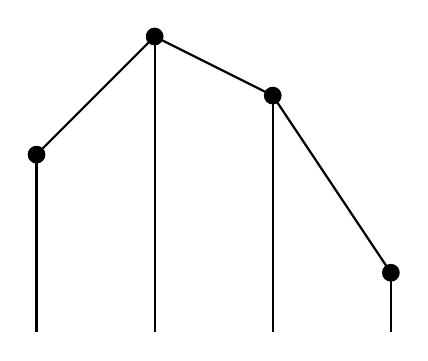
\begin{tikzpicture}[scale = 1.5]
    \def \valY{{2, 4, 3, 0.5}}

    \foreach \x in {0,...,3}{
        \pgfmathsetmacro\asInt{int(\valY[\x])}
        \pgfmathsetmacro\r{(\asInt+1)/2}
        \draw[thick, black, -](\x,0) -- (\x,\r);
        \draw[fill = black](\x,\r) circle (2pt);
        
        \pgfmathsetmacro\nextx{\x==3 ? \x : \x+1}
        \pgfmathsetmacro\nextAsInt{int(\valY[\nextx])}
        \pgfmathsetmacro\nextR{(\nextAsInt+1)/2}
        \draw[thick, black, -](\x,\r) -- (\nextx,\nextR);
    }
\end{tikzpicture}
    }
    \subfloat[\centering Bikubisch \protect\footnotemark]{
        %Berechnet mit https://tools.timodenk.com/cubic-spline-interpolation

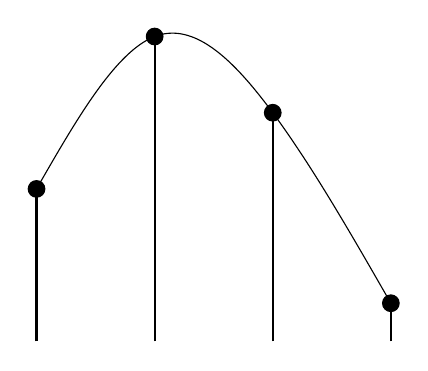
\begin{tikzpicture}[scale = 1.5]
    
        \pgfmathsetmacro\rEins{(+-0.7*0^3+1.32e-62*0^2+2.7*0^1+2*0^0)/1.55}
        \draw[thick, black, -](0,0) -- (0,\rEins);
        \draw[fill = black](0,\rEins) circle (2pt);

        \pgfmathsetmacro\rZwei{(+-0.7*1^3+1.32e-62*1^2+2.7*1^1+2*1^0)/1.55}
        \draw[thick, black, -](1,0) -- (1,\rZwei);
        \draw[fill = black](1,\rZwei) circle (2pt);

        \pgfmathsetmacro\rDrei{(+0.5*2^3+-3.6*2^2+6.3*2^1+0.8*2^0)/1.55}
        \draw[thick, black, -](2,0) -- (2,\rDrei);
        \draw[fill = black](2,\rDrei) circle (2pt);

        \pgfmathsetmacro\rVier{(+0.2*3^3+-1.8*3^2+2.7*3^1+3.2*3^0)/1.55}
        \draw[thick, black, -](3,0) -- (3,\rVier);
        \draw[fill = black](3,\rVier) circle (2pt);


    \draw[domain=0:1, smooth, variable=\x, black] plot ({\x}, {(+-0.7*\x^3+1.32e-62*\x^2+2.7*\x^1+2*\x^0)/1.55});
    \draw[domain=1:2, smooth, variable=\x, black] plot ({\x}, {(+0.5*\x^3+-3.6*\x^2+6.3*\x^1+0.8*\x^0)/1.55});
    \draw[domain=2:3, smooth, variable=\x, black] plot ({\x}, {(+0.2*\x^3+-1.8*\x^2+2.7*\x^1+3.2*\x^0)/1.55});
\end{tikzpicture}
    }
    \caption[BilinearBikubisch]{Vergleich Bilinear und Bikubisch}
\end{figure}
\footnotetext{Funktion mit \url{https://tools.timodenk.com/cubic-spline-interpolation} erstellt}

\medskip
Um die beste Qualität bei dem runterskalieren zu erhalten, wird das Bild häufiger skaliert. Dies verwaltet die imgskalr library. Das Bild wird wiederholt um $\frac{1}{7}$ seiner Breite und Höhe verkleinert. Der Wert wurde nicht mathematisch berechnet, sondern wurde durch testen herausgefunden.\cite[Scalr.java Zeile 2221]{Scalr:Kalla}

\begin{figure}[h]
    \centering
    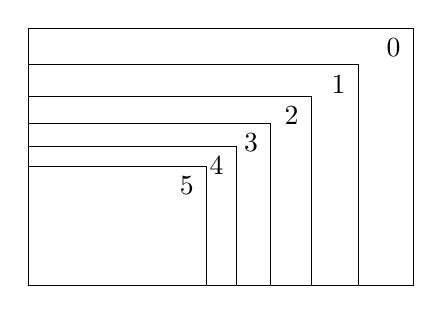
\begin{tikzpicture}[scale = 0.1]
    \def \xy {{{4890,3263},
               {4192,2797},
               {3594,2398},
               {3081,2056},
               {2641,1763},
               {2264,1512}}}

    \foreach \x in {0,...,5}{
        \pgfmathsetmacro\width{int(\xy[\x][0])/100}
        \pgfmathsetmacro\height{int(\xy[\x][1])/100}
        \draw[black](0,0)--(\width,0)--(\width,\height)--(0,\height)--(0,0);
        \node[] at (\width-2.5,\height-2.5) (a) {\x};
    }

\end{tikzpicture}
    \caption[Inkrementell]{Inkrementelles Skalieren}
\end{figure}

\newpage
%Die Laufzeitanalyse
\section{Laufzeitanalyse}
\subsection{Einleitung}
Um die Effizienz des Programms beurteilen zu können, werde ich die einzelnen Algorithmen betrachten. Dazu werde ich Das erstellen einer Datenbank, berechnen der durchschnittlichen Farbe, skalieren der Bilder und das berechnen der besten Bilder vergleichen. Der Test kann mit einer UI im Programm durchgeführt werden. Es wird ein Test mehrfach durchgeführt und bei jedem neuem Durchgang die Anzahl an Bildern erhöht. Das Testen kann mit generierten Bildern und mit zufälligen Bildern der Internetseite ``https://picsum.photos'' durchgeführt werden. Alle folgenden Tests werden mit zufälligen Bildern durchgeführt, da diese die echte Benutzung am besten Simulieren. Bei den Generierten Bildern sinken die Berechnungszeiten stark, da weniger Farbkomplexität gegeben ist. Bei jeder Simulation wird auch der benötigte Arbeitsspeicher gespeichert, da das Programm sehr Arbeitsspeicher intensiv werden kann. Die Laufzeit des Berechnen der durchschnittlichen Farbe, das erstellen einer Datenbank und das berechnen der besten Bilder ist Linear. $O(n)$ mit der Anzahl der Bilder als $n$. Die Laufzeit des Skalieren ist abhängig von dem genutzten Algorithmus.
\begin{figure}[h]
    \centering
    \subfloat[\centering Datenbank]{
        \begin{tikzpicture}[scale = 0.85]
            \begin{axis}[tick label style={
                /pgf/number format/fixed,
                /pgf/number format/fixed zerofill,
                /pgf/number format/precision=1
            }, legend pos=north west, no markers, legend style={nodes={scale=0.7, transform shape}}]
                \addplot table [x=x, y=time, col sep=semicolon] {./images/Simulationen/Database_1.000x10.000.csv};
                \addlegendentry{Zeit in ns}
                \addplot table [x=x, y=ram, col sep=semicolon] {./images/Simulationen/Database_1.000x10.000.csv};
                \addlegendentry{Ram in Byte}
            \end{axis}
        \end{tikzpicture}
        \label{DatenbankGraph}
    }
    \subfloat[\centering durchschnittliche Farbe]{
        \begin{tikzpicture}[scale = 0.85]
            \begin{axis}[tick label style={
                /pgf/number format/fixed,
                /pgf/number format/fixed zerofill,
                /pgf/number format/precision=1
            }, legend pos=north west, no markers, legend style={nodes={scale=0.7, transform shape}}]
                \addplot table [x=x, y=time, col sep=semicolon] {./images/Simulationen/averageColor_500x50_500x500_Ultra.csv};
                \addlegendentry{Zeit in ns}
                \addplot table [x=x, y=ram, col sep=semicolon] {./images/Simulationen/averageColor_500x50_500x500_Ultra.csv};
                \addlegendentry{Ram in Byte}
            \end{axis}
        \end{tikzpicture}
        \label{DurchschnittlicheFarbeGraph}
    }
    \hspace{0mm}
    \subfloat[\centering skalieren der Bilder]{
        \begin{tikzpicture}[scale = 0.85]
            \begin{axis}[tick label style={
                /pgf/number format/fixed,
                /pgf/number format/fixed zerofill,
                /pgf/number format/precision=1
            }, legend pos=north west, no markers, legend style={nodes={scale=0.7, transform shape}}]
                \addplot table [x=x, y=time, col sep=semicolon] {./images/Simulationen/scalingImages.csv};
                \addlegendentry{Bilinear(ns)}
                \addplot table [x=x, y=time, col sep=semicolon] {./images/Simulationen/scalingImagesBikubisch.csv};
                \addlegendentry{Bikubisch(ns)}
                \addplot table [x=x, y=ram, col sep=semicolon] {./images/Simulationen/scalingImages.csv};
                \addlegendentry{Bilinear(Byte)}
                \addplot table [x=x, y=ram, col sep=semicolon] {./images/Simulationen/scalingImagesBikubisch.csv};
                \addlegendentry{Bikubisch(Byte)}
            \end{axis}
        \end{tikzpicture}
        \label{SkalierenGraph}
    }
    \subfloat[\centering berechnen der besten Bilder]{
        \begin{tikzpicture}[scale = 0.85]
            \begin{axis}[tick label style={
                /pgf/number format/fixed,
                /pgf/number format/fixed zerofill,
                /pgf/number format/precision=1
            }, legend pos=north west, no markers, legend style={nodes={scale=0.7, transform shape}}]
                \addplot table [x=x, y=time, col sep=semicolon] {./images/Simulationen/computation.csv};
                \addlegendentry{Zeit in ns}
                \addplot table [x=x, y=ram, col sep=semicolon] {./images/Simulationen/computation.csv};
                \addlegendentry{Ram in Byte}
            \end{axis}
        \end{tikzpicture}
        \label{BesteBilderGraph}
    }
    
    \caption[BilinearBikubisch]{Vergleich Bilinear und Bikubisch}
\end{figure}
Test \ref{DatenbankGraph} wurde von $10000$ bis $10000000$ Bilder durchgeführt. Die Zeit erhöht sich um 1250ns pro Bild. Die Arbeitsspeichernutzung erhöht sich um 87Byte pro Bild. Die Arbeitsspeichernutzung ist dabei auch stark von der Länge des Speicherortes des Bildes abhängig.
\newline
Test \ref{DurchschnittlicheFarbeGraph} wurde von $1000$ bis $25000$ Bilder durchegführt. Die Bilder hatten eine größe von 500x500px. Die Laufzeit für ein Bild liegt bei 1,09ms. Für jedes weitere Bild werden 88kByte verbraucht. Beide Werte verhalten sicht linear zu der Anzahl der Bilder.
\newline

ÜBERPRÜFEN!!!!

Das Skalieren der Bilder in \ref{SkalierenGraph} wurde jeweils mit einem Bilinearen Algorithmus und einem Bikubischen Algorithmus durchgeführt. Dazu wurden 500x500px große Bilder auf 100x70px scaliert. Der Test wurde mit $1000$ Bildern gestartet und mit $12500$ beendet. Es ist zu erkennen, dass nur ein geringer Laufzeitunterschied von $\Delta t = 4,2ms - 3,7ms = 0,5ms$ zwischen den beiden Algorithmen besteht. Dieser geringe unterschied kommt daher, dass beide Algorithmen sich sehr ähnlich verhalten. Der Unterscheid liegt lediglich bei der komplexeren Berechnung in dem Bikubischem Algorithmus, welche nur einen Teil der Laufzeit beansprucht.

\end{document}